\hypersetup{colorlinks=true, linkcolor=blue, citecolor=red}

\chapter{Dataset analysis} \label{chap:dataset_analysis}

    In this chapter, the dataset used in this thesis is analyzed. The data collection methodology is described, along with the recording setup. The data structure and attributes are presented, along with the participants characteristics. Finally, the data processing steps are described.

    \section{Data collection methodology}
        
        Data used in this thesis is collected at the Waterford Hospital in Ireland as part of a Fear of Falling study conducted on a group of 22 elderly individuals.  A Microsoft Kinect sensor is used to record the movements performed following a recording setup. 

        \subsection{Microsoft kinect}

                The first generation of the Kinect sensor, Kinect V1 in Figure \ref{fig:kinect_sensor}, is a motion sensing input device developed by Microsoft and first released in 2010 for game consoles and Microsoft Windows PCs \cite{xu_validity_2015}. A new version of the Kinect sensor, Kinect V2, is released in 2014, with improved hardware and software \cite{cruz_kinect_2012}. 

                \begin{figure}[H]
                    \centering
                    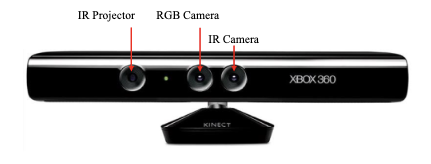
\includegraphics[width=0.6\textwidth]{./resources/images/kinect/kinect.png}
                    \caption{Microsoft Kinect Sensor.}
                    \label{fig:kinect_sensor}
                \end{figure}

                    \subsubsection{Kinect sensor} 

                        The Kinect Sensor is a horizontal bar connected to a small base with a motorized pivot and is designed to be positioned lengthwise above or below the video display. The device features a color camera, an infrared (IR) emitter, an IR depth sensor, an engine for tilting, a microphone array, and a LED light \cite{abbasi_motion_2021}. The sensor is capable of sending three types of data: color images, 3D depth images, and bone information corresponding to the 3D imaging field \cite{zheng_cg-recognizer_2022}\cite{acis_classification_2023}. Along with its open source libraries, the Kinect system has helped to develop a wide range of applications in the fields of computer vision, robotics, and human computer interaction. This is because the Kinect offers a cost effective and broadly accessible metod for capturing 3D human motion data, with the advantage of allowing users to interact with the system without the need for any physical devices \cite{gowing_kinect_2014}.
                
                        \begin{figure}[H]
                            \centering
                            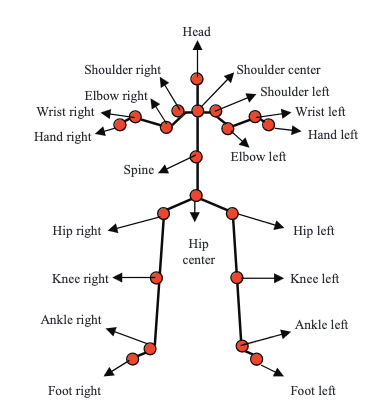
\includegraphics[width=0.6\textwidth]{./resources/images/kinect/joints.png}
                            \caption{Skeletal joints recognized by the Kinect sensor \cite{jais_review_2015}.}
                            \label{fig:kinect_sensor_v2}
                        \end{figure}

                    \subsubsection{PyKinect2}
                        PyKinect2 is a Python library for Microsoft's Kinect V2 sensor. It provides a wrapper for the Kinect for Windows SDK 2.0, which allows for the use of the sensor in Python. The library abstracts the complex functionality of the hardware into an easy to use API. Key feature include:
                        \begin{itemize}
                            \item \textbf{Skeletal tracking}: detects and tracks human bodies, providing joint positions and orientations.
                            \item \textbf{Color, depth, and infrared streams}: Accesses raw sensor streams for visual processing or analysis.
                            \item \textbf{Coordinate mapping}: translates between different spatial representations. Such as mapping skeletal joints to color or depth images for overlay visualization.
                        \end{itemize}
                        The library is a great bridge between the Kinect sensor and the Python programming language, allowing for the use of the sensor in a variety of applications \cite{GitHubKinectPyKinect2}.
               
                        \newpage
                        
        \subsection{Recording setup}

                    The patient's data recording setup illustrated in Figure \ref{fig:kinect_setup} consists of consumer-level hardware (a laptop, a Kinect V2 depth camera, an external webcam, and a smartphone) and a dedicated application developed within the project. 
                    Once launched, the operator can display a sample stimulus on an external monitor to show the target movements to the patient (\textit{1. Stimulus playback}) so they can repeat (\textit{2. patient performs movement}) them by selecting one of them from a list in the appplication.
                    Then, by pressing the "\textit{record}" button (\textit{3. record/analyse skeleton + rgb + accelerometer}), the recording of the patient's full body movement can be started. 
                    The application stores the recorded patient's movement files in a separate folders, naming them based on their patient ID, movement ID, and repetition ID.

                    \begin{figure}[H]
                        \centering
                        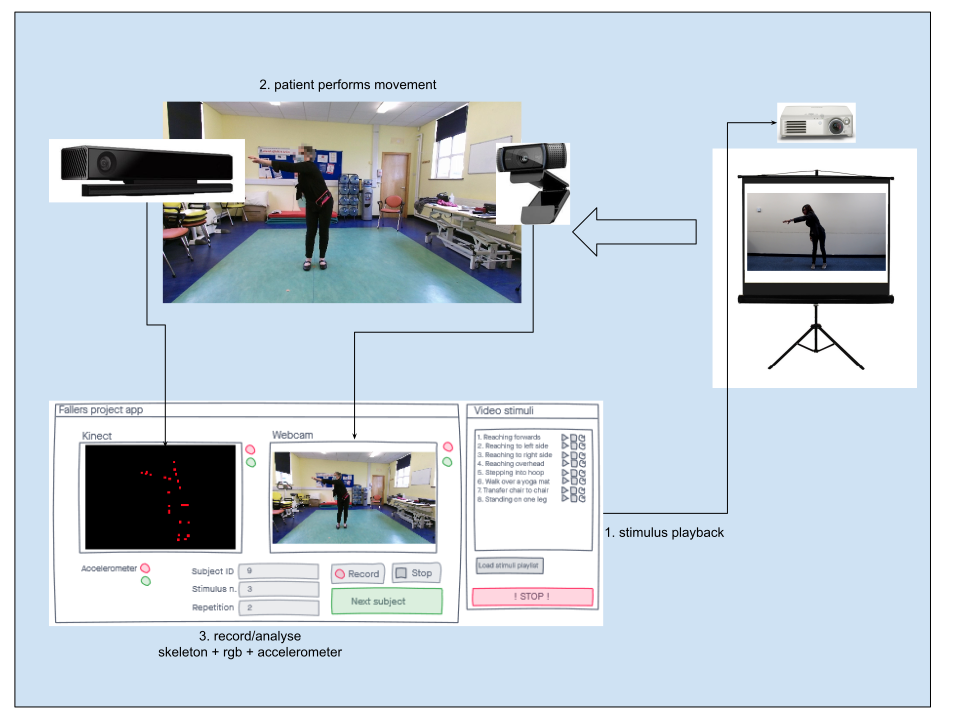
\includegraphics[width=0.9\textwidth]{./resources/images/kinect/setup.png}
                        \caption{Setup used at the Waterford Hospital for data collection.}
                        \label{fig:kinect_setup}
                    \end{figure}
                    
                    %\newpage 

                    The full body capture mainly relies on the PyKinect library \cite{GitHubKinectPyKinect2}.
                    The library provides functions for getting the patient's body segment's position and rotation 25 times per second. The application gets the data and stores it as a multi dimensional time series (one per body segment and coordinate type) in CSV files like the one displayed in Figure \ref{fig:csv_structure}.
                    \newpage
                    \begin{figure}[H]
                        \centering
                        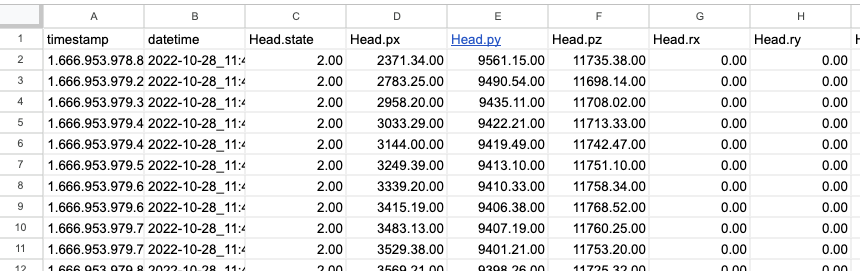
\includegraphics[width=1.0\textwidth]{./resources/images/other/data.png}
                        \caption{Example of a CSV file containing the Kinect skeleton data.}
                        \label{fig:csv_structure}
                    \end{figure}

                    The accelerometer is captured via a smartphone running an app streaming 3D gyroscope data at 50 frames per second. Again, the application on the computer stores it as a multi dimensional time series (one per rotation axis). The communication between the smartphone and the computer is based on a wireless network and the Open Sound Control (OSC) protocol \cite{wright_open_nodate}.
    
    \section{Data structure and attributes}
            
            Data used in this thesis consists of a series of CSV files, each containing 3D coordinates of the joints of a participant performing a movement. The total number of csv files is \textbf{637}. In Figure \ref{fig:dataset_files} the distribution of the csv files between the movements is presented with a median of \textbf{68} files per movement.

            \begin{figure}[H]
                \centering 
                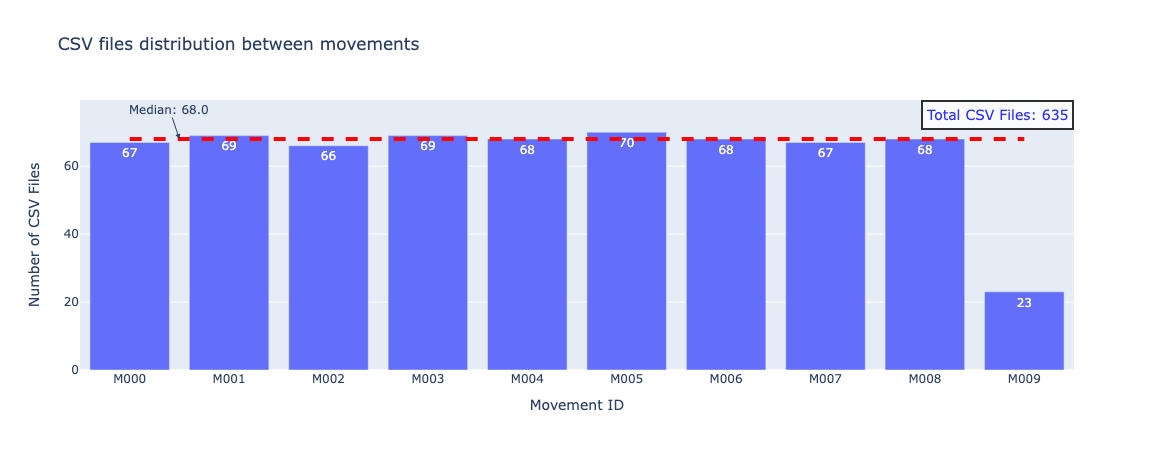
\includegraphics[width=1.0\textwidth]{./resources/plots/participants/csv_files.png}
                \caption{CSV files distribution between the movements. \textit{M009} is the only movement with less than 68 files due to it not being performed multiple times by the participants.}
                \label{fig:dataset_files}
            \end{figure}
        
            Dataset is organized in a directory structure. Each patient has a folder named with their ID (\textit{Participant-ID}) and inside there are 10 folders for each movement, named with the movement ID (\textit{M-XXX}). For every movement folder there is a folder for each repetition of the movement, named with the repetition ID (\textit{R-XXX}). Inside each repetition folder there is a CSV file that contains the Kinect skeleton data. In Figure \ref{fig:directory-structure} an example of the directory structure is displayed. \\
            
            \begin{figure}[htbp]
                \centering
                \begin{forest}
                for tree={
                folder,
                grow'=0,
                fit=band,
                }
                [Participants
                    [Participant-1
                        [M000
                            [R000
                                [FILE.CSV]
                            ]
                            [R001]
                            [R002]
                        ]
                    ]
                ]
                \end{forest}
                \caption{Directory structure example using the first patient and first movement in the dataset. }
                \label{fig:directory-structure}
            \end{figure}

            a CSV file is organized as a series of columns, each column represents a joint in Table \ref{tab:joints_recorded} that the Kinect sensor records. Each joint is represented by 7 columns, one for each position and rotation coordinate (x, y, z) and one for the state. The state column is used to indicate if the joint is trackd or not. Beside the joints columns, there are 2 columns for the timestamp and datetime of the recording.
            
            \begin{table}[H]
                \centering
                \begin{tabularx}{1.0\textwidth}{XXXX} 
                    \toprule
                    \multicolumn{4}{c}{\textbf{Joints}} \\ 
                    \midrule
                    AnkleLeft & AnkleRight & ElbowLeft & ElbowRight \\
                    FootLeft & FootRight & HandLeft & HandRight \\ 
                    HandTipLeft & HandTipRight & Head & HipLeft \\
                    HipRight & KneeLeft & KneeRight & Neck \\
                    ShoulderLeft & ShoulderRight & SpineBase & SpineMid \\ 
                    SpineShoulder & ThumbLeft & ThumbRight & WristLeft \\
                    WristRight & & & \\
                    \bottomrule
                \end{tabularx}
                \caption{Joints processed with the PyKinect2 library.}
                \label{tab:joints_recorded}
            \end{table}

    \section{Participants characteristics}
        The participants that take part in the study are 22 elderly individuals, in Figure \ref{fig:age_distribution} the age distribution is presented, with a median age of 67 years. 
        \newpage 
        \begin{figure}[H]
            \centering
            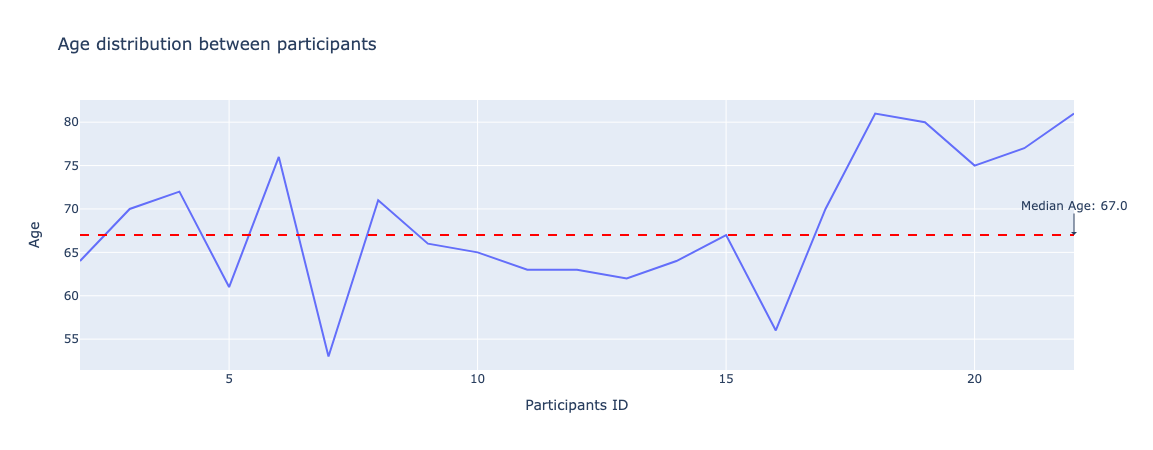
\includegraphics[width=1.0\textwidth]{./resources/plots/participants/age.png}
            \caption{Age distribution of the participants.}
            \label{fig:age_distribution}
        \end{figure}

        In Figure \ref{fig:patients_characteristics} participants characteristics are presented. \textbf{Fear of Falling} is present in \textbf{57\%} of the participants, this is a relatively high percentage, due to the study being conducted on a Fear of Falling assessment group. The gender is dominated by \textbf{females} with a \textbf{95\%} of the participants, this is also expected since most studies in the literature had mostly female participants (>50\%) \cite{mackay_fear_2021}. The education is also presented, with the majority of the participants having a \textbf{Secondary} or \textbf{Third Level} education.
        
        \begin{figure}[H]
            \centering
            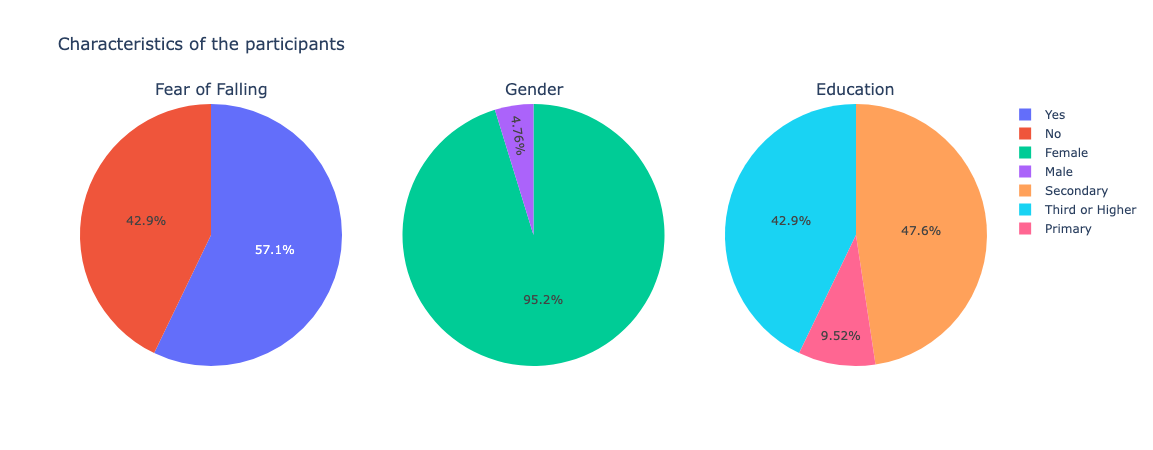
\includegraphics[width=1.0\textwidth]{./resources/plots/participants/chars.png}
            \caption{Characteristics of the participants in the study.}
            \label{fig:patients_characteristics}
        \end{figure}

        \subsubsection{What is fear of falling ?}
        
            The definition of \textbf{Fear of Falling} had various interpretations over the years. Initially, it is described as a phobic reaction to standing or walking. However, it is reclassified as a syndrome characterzied by the aftermath of a fall. As understanding developed, this fear is seen as a loss of confidence in one's balance ability. It is also further defined as an ongoing concern about falling, which leads to the avoidance of performing daily activities. Recently, it has been described as continous avoidance of activities due to the concern of falling \cite{jung_fear_2008}.
    
    \section{Movements visualization} \label{sec:movements_visualization}
        
        Kinect skeleton data comes as a series of 3D coordinates, which can be visualized in 3D space. In this section, the implementation of the movements visualization is presented. The visualization was implemented using the Python programming language and the Plotly library \cite{plotly}.

        The first step in the visualization process is to identify the set of joints to be used. In this approach, the dataset contains 25 joints but only 16 joints are used and are displayed in Table \ref{tab:joints_select}. 

        \begin{table}[H]
            \centering
            \begin{tabularx}{1.0\textwidth}{XXX}
                \toprule
                \multicolumn{3}{c}{\textbf{Joints}} \\
                \midrule
                Head & Spine Shoulder & Spine Mid \\
                Spine Base & Shoulder Right & Elbow Right \\
                Wrist Right & Shoulder Left & Elbow Left \\
                Wrist Left & Hip Right & Knee Right \\
                Ankle Right & Hip Left & Knee Left \\
                Ankle Left & & \\
                \bottomrule
            \end{tabularx}
            \caption{Selected kinect joints used for the visualization.}
            \label{tab:joints_select}
        \end{table}
        
        Once the joints are selected, the next step is to transform the data. In its original state the data is organized incorrectly for the 3D visualization, the y and z coordinates are inverted. To fix this, the y and z coordinates are swapped. \\

        After the transformation is performed, the data is ready to be visualized. Snippet \ref{lst:visualization} shows the implementation of the visualization process, it begins by extracting joint coordinates and their connections, assigning colors and sizes to major joints, and configuring the 3D layout. Animation frames are generated by iterativly capturing snapshots of joint positions and connections over time. These frames are then combined and displayed in an interactvie 3D plot, allowing the user to play the animation and rotate the plot to view the movement from different angles.

        \begin{lstlisting}[caption={Code snippet creates connecting lines between joints using their 3D coordinates, enabling visualization of joint movements.}, label={lst:visualization}, language=Python]            
    for index, row in data.iterrows():
        x_values = [row[f"{joint}.px"] for joint in joints]
        y_values = [row[f"{joint}.py"] for joint in joints]
        z_values = [row[f"{joint}.pz"] for joint in joints]
        lines = []
        for connection in connections:
            start, end = connection
            lines.append(go.Scatter3d(
                    x=[row[f"{start}.px"], row[f"{end}.px"]],
                    y=[row[f"{start}.py"], row[f"{end}.py"]],
                    z=[row[f"{start}.pz"], row[f"{end}.pz"]],))
        \end{lstlisting}
        
        \newpage

        In Figure \ref{fig:movements_visualization} a set of movements performed by the participants are presented. The movements are displayed in a 3D plot, with the x, y, and z axes representing the plot axes. 

        \begin{figure}[h]
            \begin{subfigure}{.5\textwidth}
                \centering
                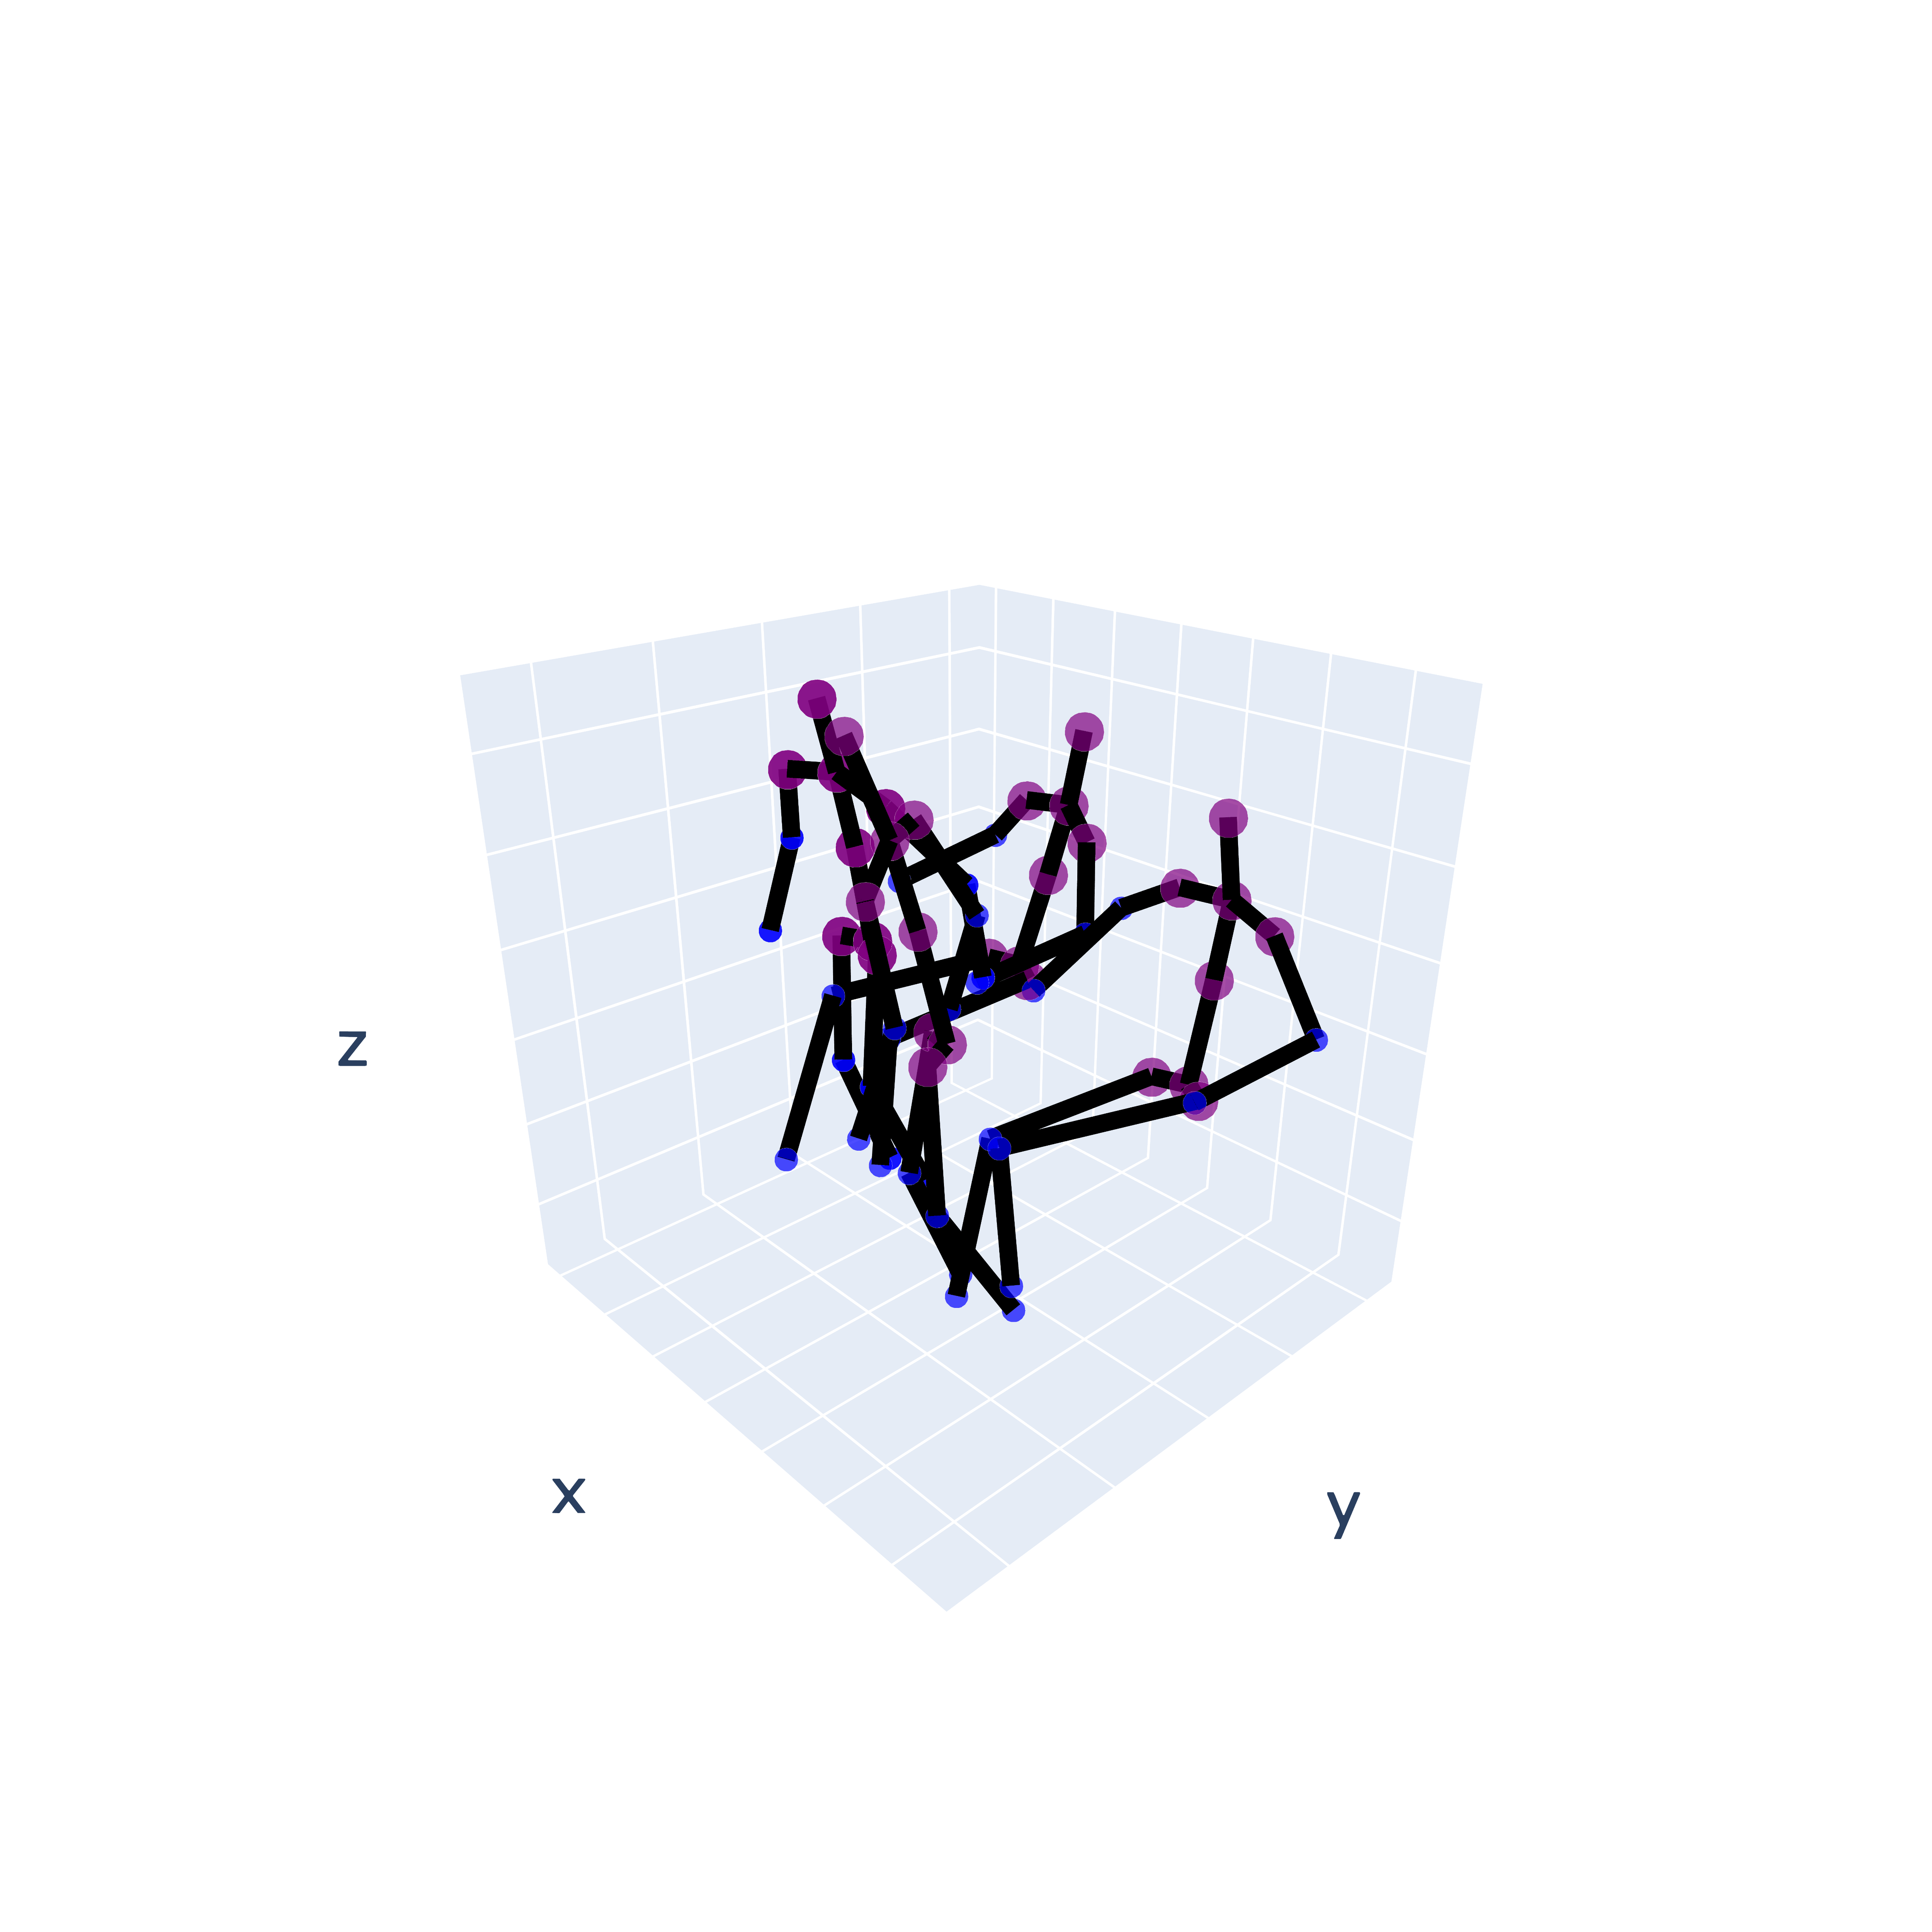
\includegraphics[width=.9\linewidth]{../src/resources/plots/movements/mov-0.png}
                \caption{Chair to Chair}
                \label{fig:mov-0}
            \end{subfigure}
            \begin{subfigure}{.5\textwidth}
                \centering
                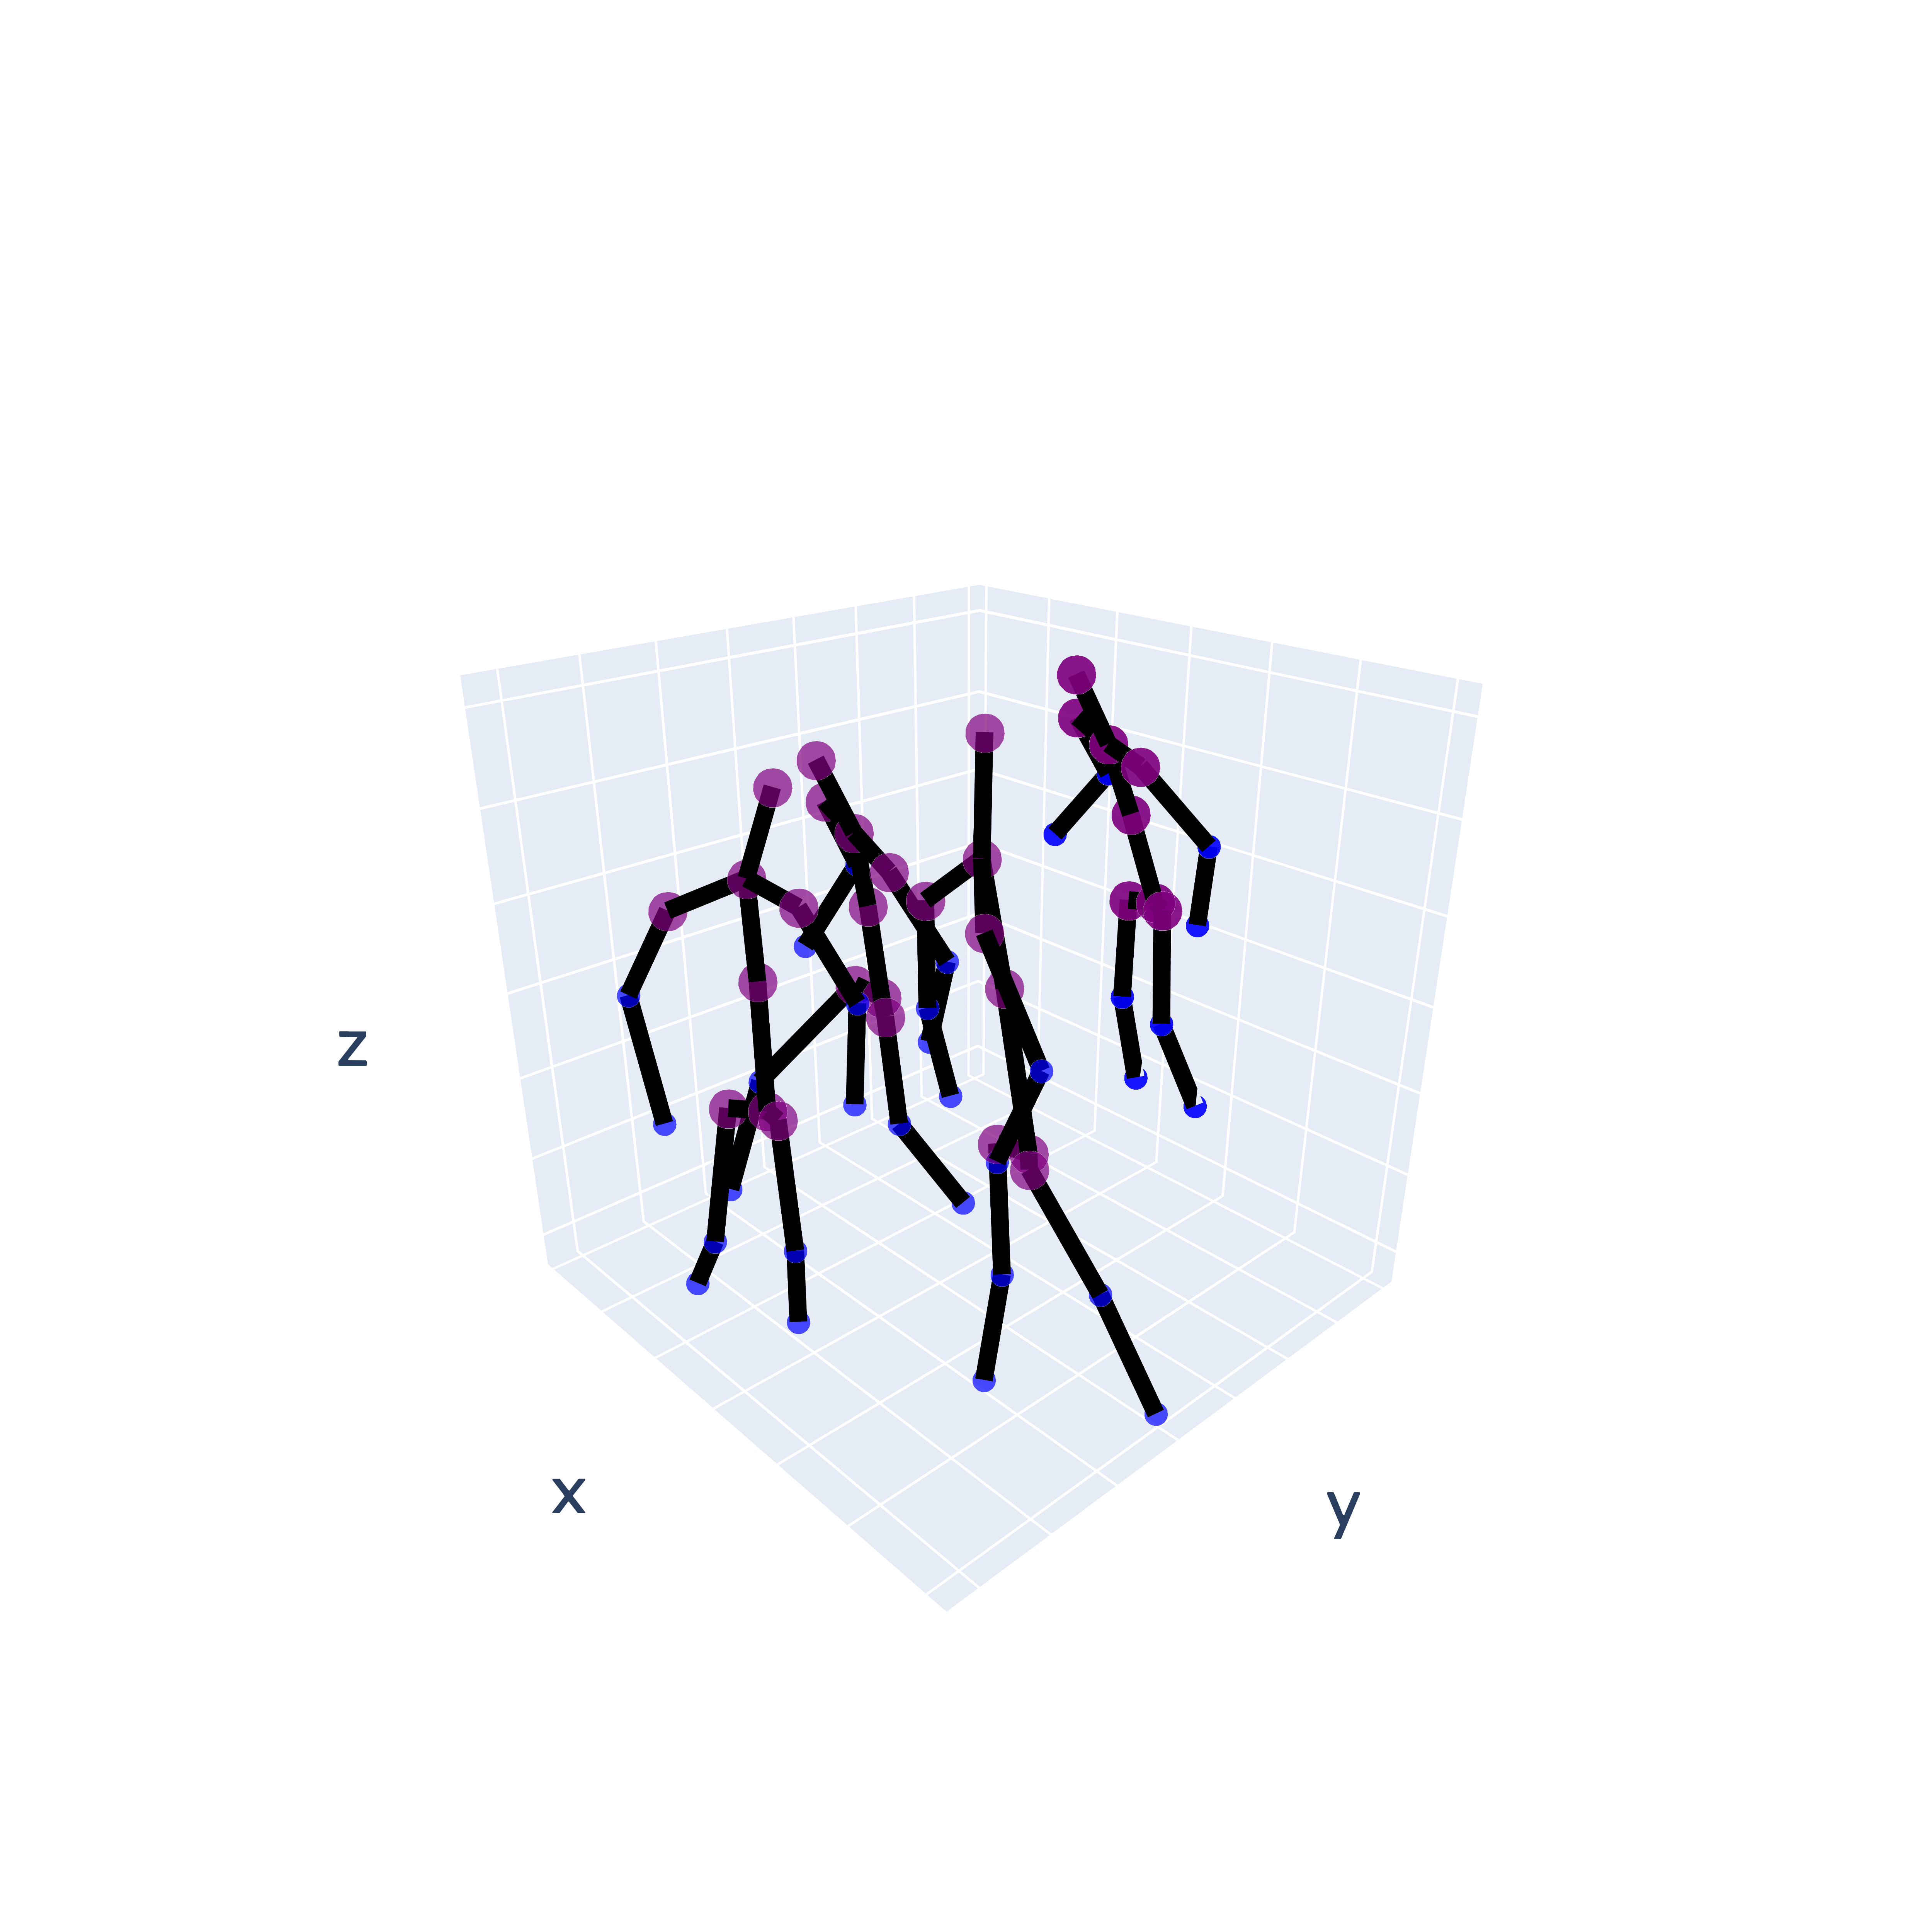
\includegraphics[width=.9\linewidth]{../src/resources/plots/movements/mov-1.png}
                \caption{Hoop Walk}
                \label{fig:mov-1}
            \end{subfigure}
            
            \begin{subfigure}{.5\textwidth}
                \centering
                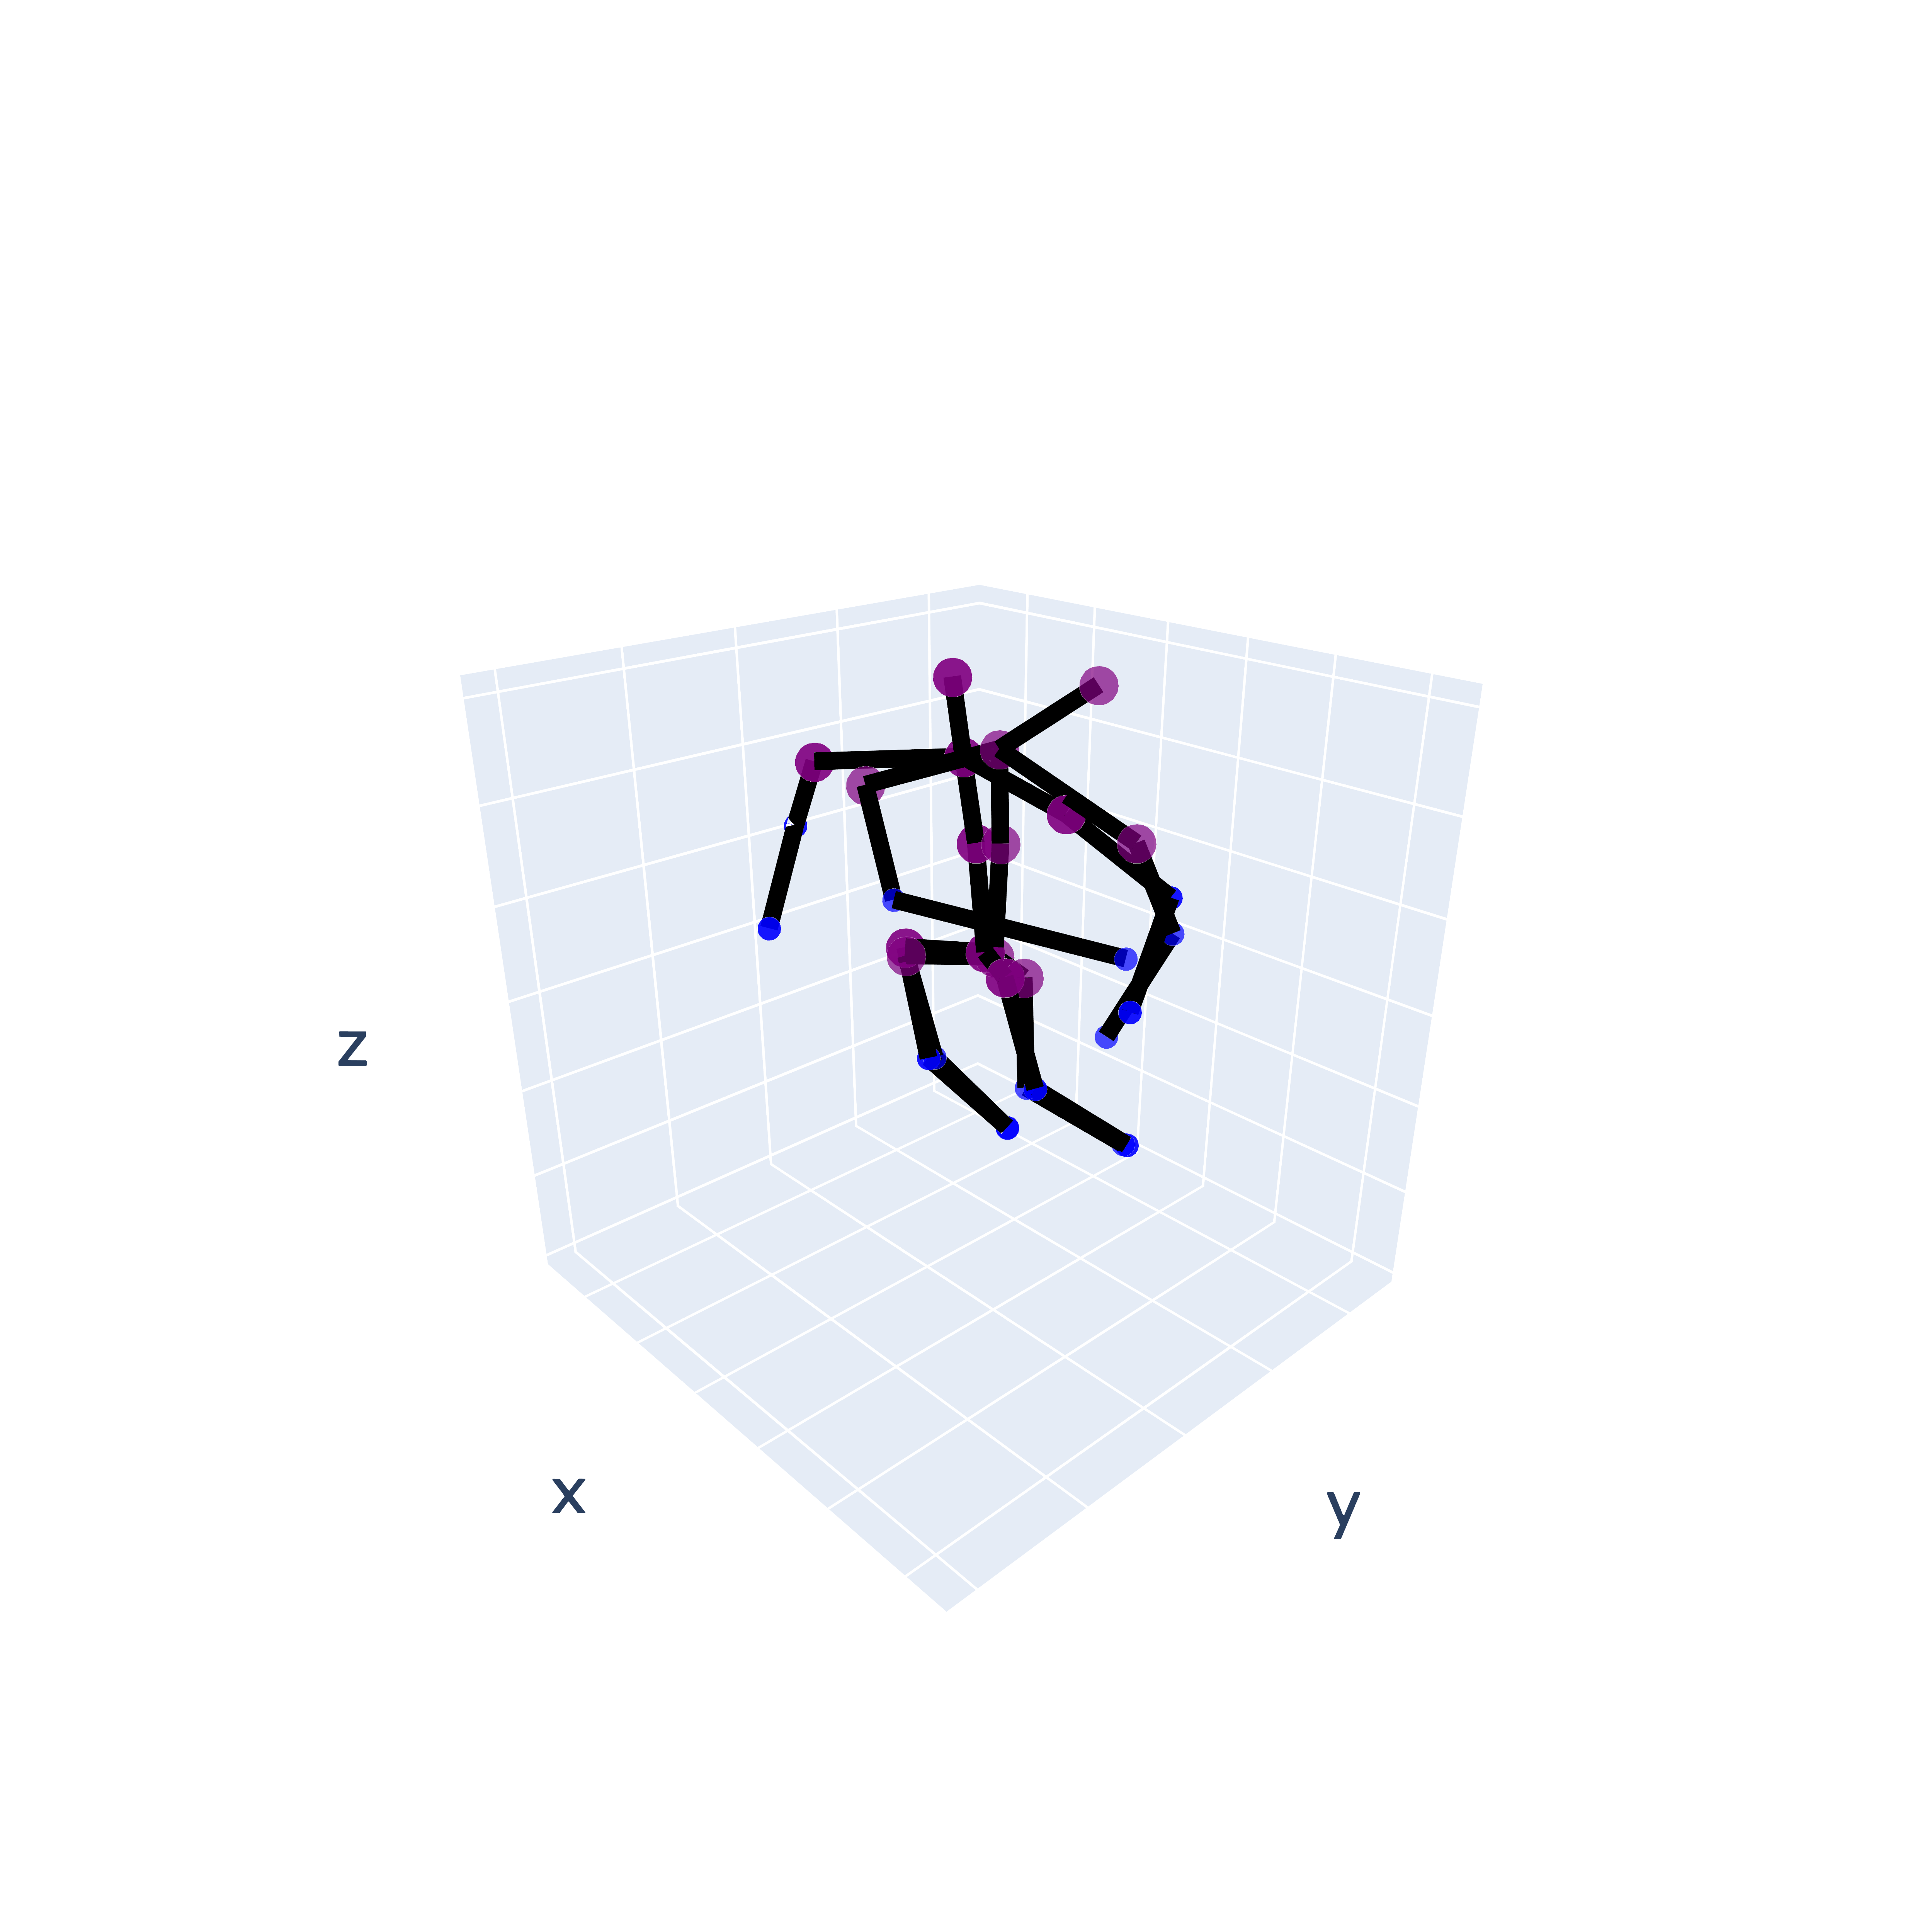
\includegraphics[width=.9\linewidth]{../src/resources/plots/movements/mov-2.png}
                \caption{Cross Reach Left}
                \label{fig:mov-2}
            \end{subfigure}
            \begin{subfigure}{.5\textwidth}
                \centering
                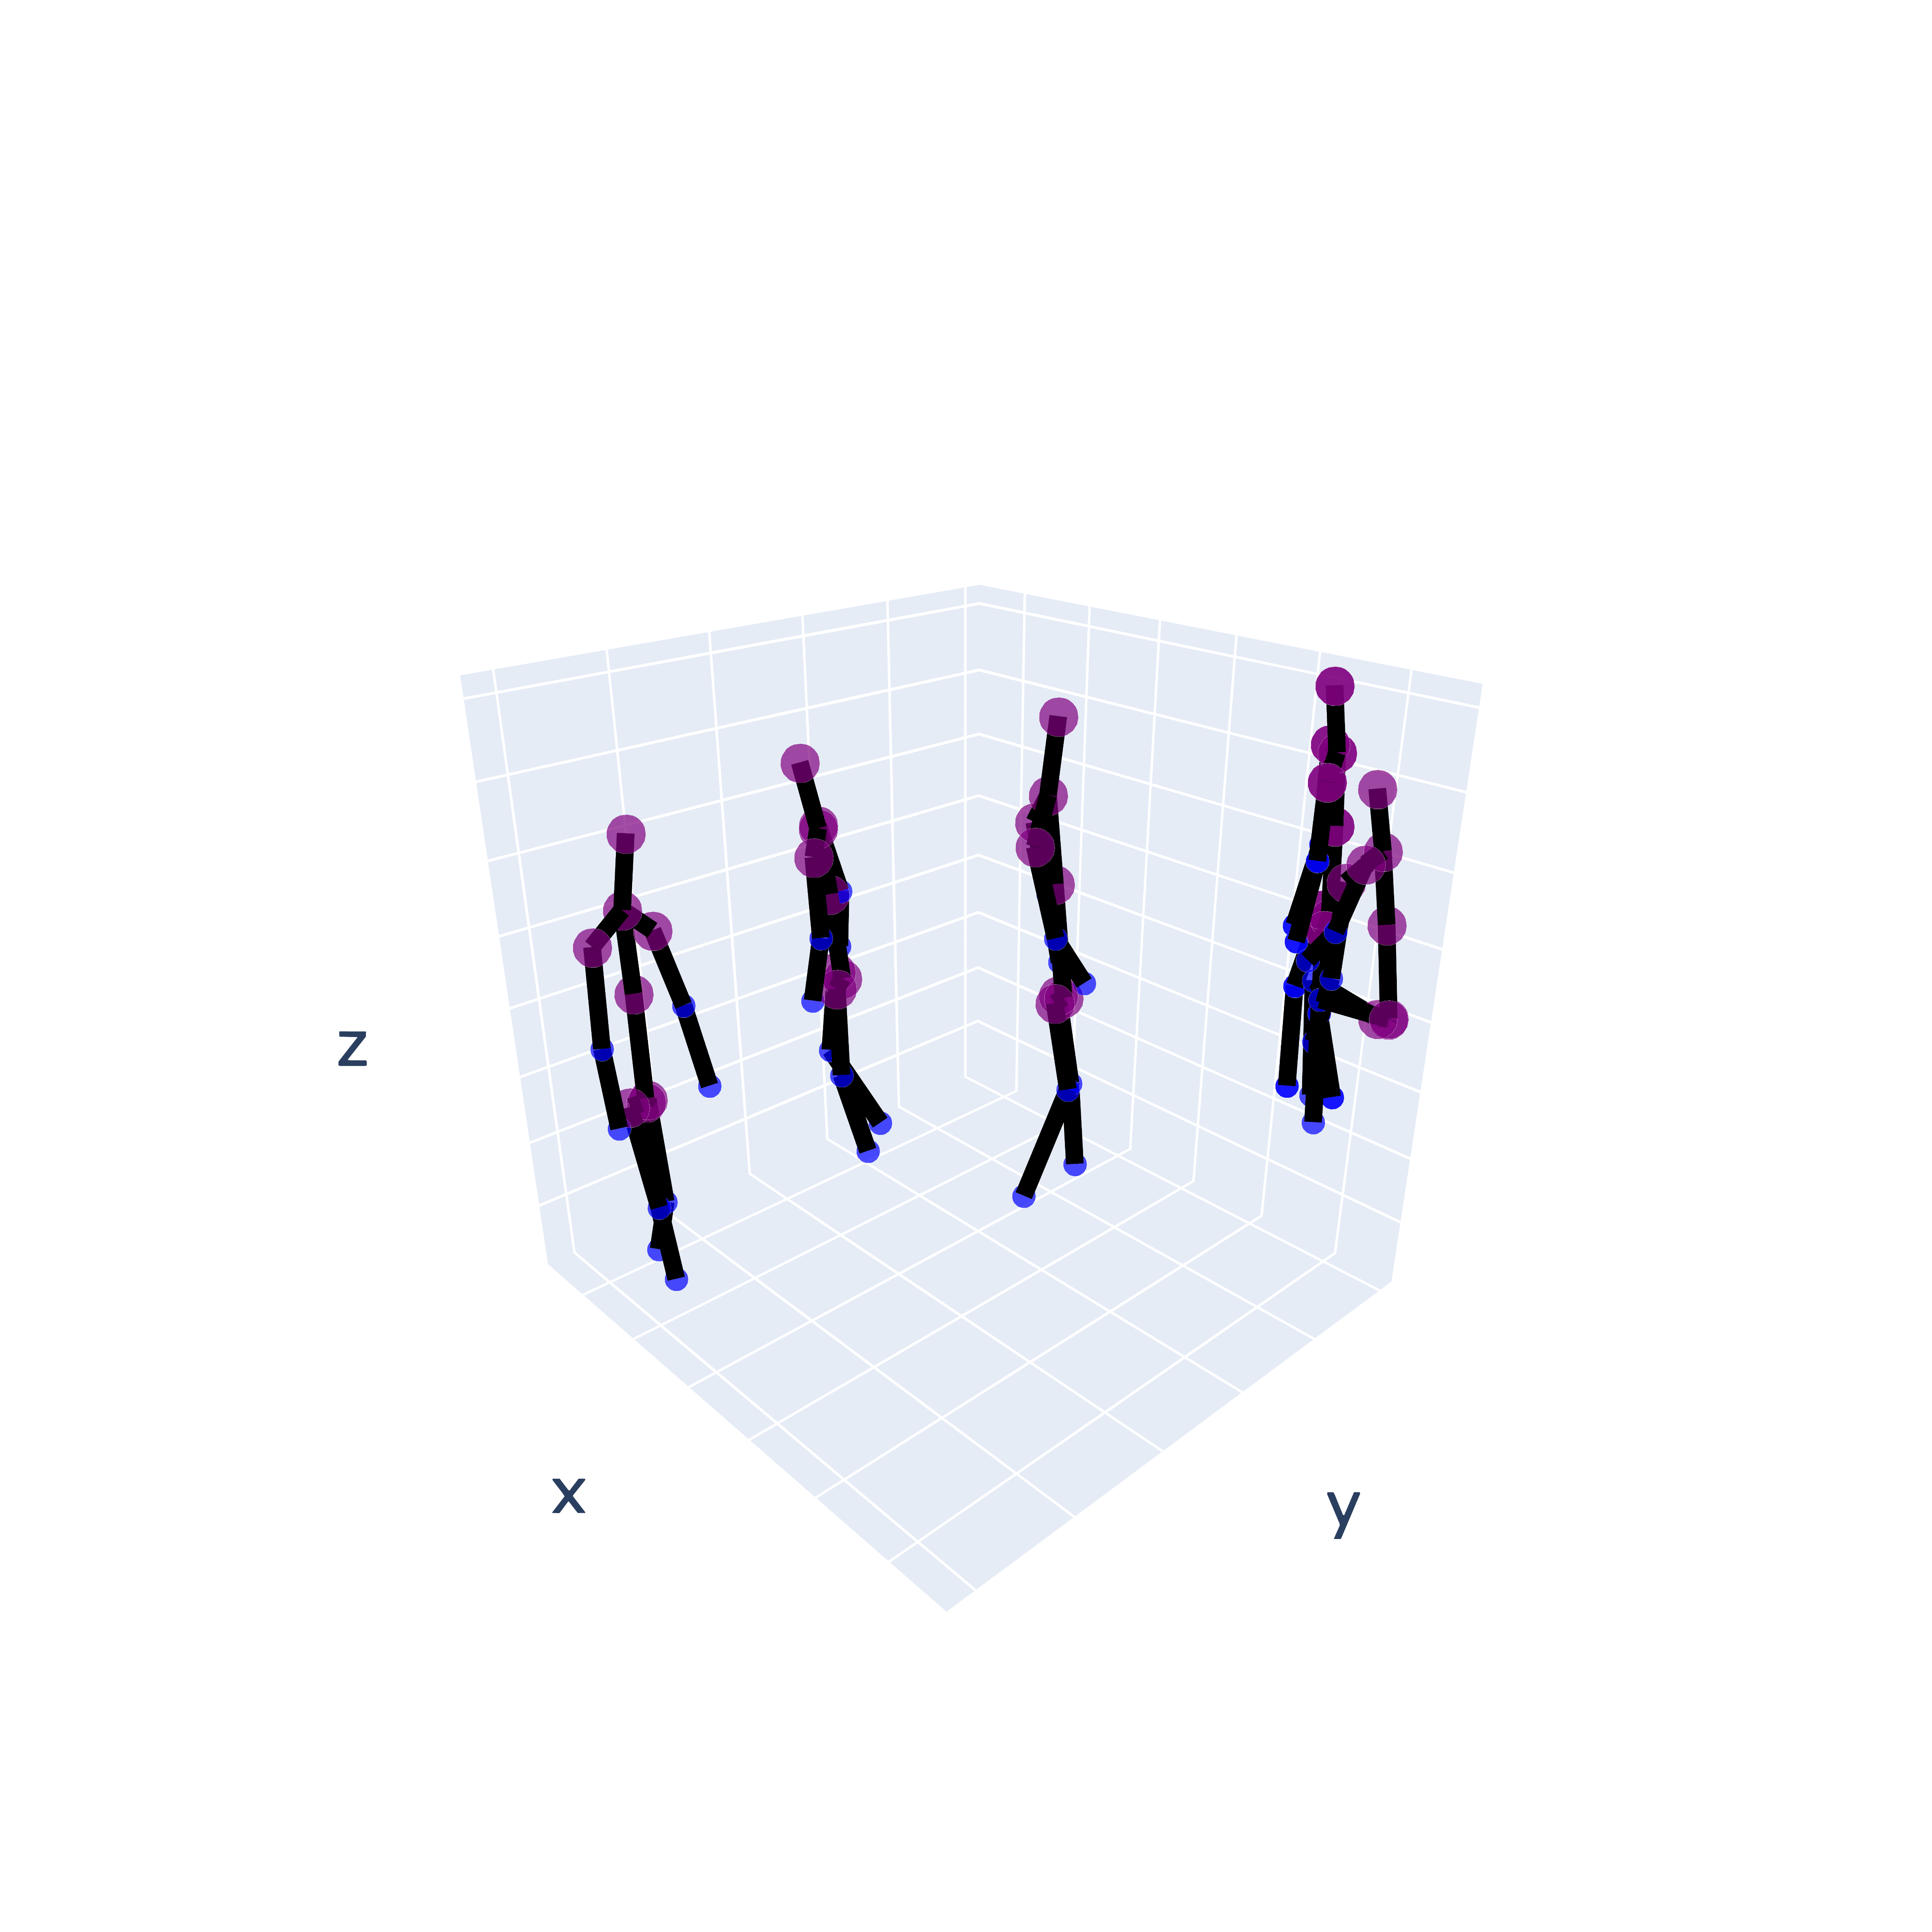
\includegraphics[width=.9\linewidth]{../src/resources/plots/movements/mov-9.png}
                \caption{Tug Walk}
                \label{fig:mov-9}
            \end{subfigure}
            
            \caption{Visualization of movements performed by the participants. Each plot is a 3D visualization containing frames that display the animation.}
            \label{fig:movements_visualization}
        \end{figure}

    \section{Data processing}

        Original dataset containing the Kinect skeleton data is processed to remove noise and outliers. This process is needed to improve the classification results. The data processing steps are described in the following sections.
        
        \subsection{Cleaning}
        
        From the original dataset a process of cleaning the data is performed. Consisting of removing the columns that contained zero values and the ones that are not needed for the classification task. The columns that are kept are listed in the Table \ref{tab:joints_select}, only the positional coordinates are kept, the state columns and rotation columns (x, y, z) are removed due to not giving any useful information for the classification task.

        \subsection{Normalization}

        Pose normalization was performed using the formula described in \cite{maudsley-barton_comparative_2017} as follow:
        \begin{equation}
            P_{n,i}(x,y,z) = P_{n,i}(x,y,z)-P_{spinebase,1}(x,y,z)
            \label{eq:pose_normalization}
        \end{equation}

        Equation \ref{eq:pose_normalization} is used to normalize the pose of a participant performing a movement. The pose is normalized by subtracting the coordinates of the spine base joint in the first frame from the coordinates of all the joints in the dataframe. This is done to remove the effect of the position of the participant in the recording setup and align all the frames to the same position. 

        \subsection{Transformation}

        Once the data cleaning and normalization is performed, the data is transformed into a format that can used for a classification task. Using the Scikit Learn library \cite{sklearn_api}, \textbf{MinMaxScaler} is used to scale the data between 0 and 1 then \textbf{StandardScaler} is used to standardize the data. After this process the data is ready for a Machine Learning model.

\cleardoublepage